% AASTeX v6.2
%\documentclass[preprint]{aastex62}

% ApJ Format
\documentclass[iop,revtex4,twocolumn,apj,numberedappendix,appendixfloats]{emulateapj}
\usepackage{apjfonts}
% Hyperlinks & Bookmarks
\usepackage[pagebackref=false,colorlinks=true,citecolor=blue,linkcolor=blue,breaklinks=true,bookmarks=true]{hyperref}
\usepackage{amsmath}
\usepackage{comment}

% Units
\newcommand{\kms}{km~s$^{-1}$}
\newcommand{\msun}{$M_{\odot}$}
\newcommand{\msunyr}{$M_{\odot}~{\rm yr}^{-1}$}
\newcommand{\lsun}{$L_{\odot}$}
\newcommand{\ergs}{erg~s$^{-1}$}
\newcommand{\cmsq}{cm$^{-2}$}
\newcommand{\um}{$\mu$m}
\newcommand{\uJy}{$\mu$Jy}
\newcommand{\sqdeg}{deg$^2$}
\newcommand{\lx}{$L_{\rm X}$}
\newcommand{\lmir}{$L_{\rm 12\mu m}$}
\newcommand{\loiii}{$L_{\rm [OIII]}$}
% Emission lines
\newcommand{\Ha}{H$\alpha$}
\newcommand{\Hb}{H$\beta$}
\newcommand{\OII}{[O\,{\sc ii}]}
\newcommand{\OIIlam}{[O\,{\sc ii}]\,$\lambda$3727}
\newcommand{\SII}{[S\,{\sc ii}]}
\newcommand{\OIII}{[O\,{\sc iii}]}
\newcommand{\OIIIlam}{[O\,{\sc iii}]\,$\lambda$5007}
\newcommand{\NII}{[N\,{\sc ii}]}
\newcommand{\NeIII}{[Ne\,{\sc iii}]}
% special 
\newcommand{\nod}{\nodata}

\newcommand{\angstrom}{\mbox{\normalfont\AA}}
\newcommand{\reff}{$R_{\rm eff}$}
\newcommand{\ewha}{EW(H$\alpha$)}
\newcommand{\logm}{log({\it M}/M$_{\odot}$)}
%\newcommand{\arcsec}{\prime\prime}
\newcommand{\simard}{Simard+11}

% citations
\defcitealias{Fu18}{Paper I} 

\usepackage{epstopdf}

\begin{document}

\title{
SDSS-IV MaNGA: Mass Independent Star Formation Enhancement in Close Galaxy Pairs
}

\author{
Joshua L. Steffen\altaffilmark{1}, 
Hai Fu\altaffilmark{1}, and 
MaNGA Team 
}
\altaffiltext{1}{Department of Physics \& Astronomy, The University of Iowa, 203 Van Allen Hall, Iowa City, IA 52242}

\begin{abstract}
We study the spatial profile of the star formation rate (SFR) in a sample of {\it 160} interacting galaxies within the SDSS-IV MaNGA survey. We find that the specific star formation rate (sSFR) is centrally (e.g. within a single effective radius) enhanced in interacting galaxies by $\sim$0.25 $\pm$ 0.1 but that there is no enhancement or suppression in their disks. We split the radial profile into five separate stellar mass bins from \logm\ $=$ 9.0$-$11.5 and find that the sSFR enhancement has no dependence on the stellar mass of the paired galaxies. Within one effective radius, the sSFR enhancement in each of the mass bins falls within $\sim$0.1 dex of the median profile for the whole pair sample. We then use a second method to compare paired galaxies and control galaxies where each paired galaxies is matched to a set of 20 control galaxies based on stellar mass and redshift. The sSFR enhancements found are still mass independent, reinforcing the idea that low mass galaxies experience the same level of enhancement to their star formation rate as high mass galaxies. Since the merger induced sSFR enhancement is constant over stellar mass, low mass galaxies will experience a higher fractional mass growth rate of 1$-$7\%, assuming a constant burst merger induced star formation over a 1 Gyr period. This indicates that merger induced star formation has a significant impact on the mass evolution of low mass galaxies. 

\end{abstract}

\keywords{galaxies: star formation --- galaxies: nuclei --- galaxies: interactions --- galaxies: mass evolution}

%%%%%%%%%%%%%%%%%%%%%%%%%%%%%%%%%%%%%%%%%%%%%%%%%%%%
\section{Introduction}\label{sec:intro}

%%%Galaxy Evolution%%%
In the $\Lambda$CDM model, galaxy evolution is a hierarchical process. In this model, massive galaxies are the product of several past merger events of smaller galaxies. In fact, cosmological hydrodynamical simulations have shown that repeated merger events may be responsible for as much as $\sim$60\% of stellar mass in massive galaxies like M87 (e.g. \citet{Rodriguez-Gomez:2016}; \citet{Pillepich:2018}). 

%%%Simulations%%%
The internal dynamics of these interacting galaxies were first modeled in the seminal work, \citet{Toomre:1972}. Since then, hydrodynamical simulations have expanded upon the N-body simulations of \citet{Toomre:1972} by modeling gas-dynamics within the galaxies. These simulations show how barred structures develop within the disks of the interacting galaxies due to the tidal torques between them \citep{Barnes:1991}. As the bars form, the gases within the galaxy's disk lose angular momentum and get funneled into the centers of the galaxies. 

When the gas-inflows impact upon the gases in the nucleus of galaxy a burst of new star formation in triggered \citep{Barnes:1996, Mihos:1996}. These gas inflows will also bring metal-poor gases from the disk into the center of the galaxy which can dilute the central metallicity \citep{Rupke:2010, Perez:2011, Scudder:2012}. The gas-inflows may also be able to make it into very center of the galaxy and trigger supermassive black hole (SMBH) accretion \citep{Capelo:2017}. 

%%%Observations%%%
Centrally enhanced star formation has also been observed in galaxy pairs with large spectroscopic surveys including; CfA2 (Center of Astrophysics Redshift Survey)  \citep{Barton:2000, Woods:2006}, 2dF (Two Degree Field) \citep{Lambas:2003}, AEGIS (All-Wavelength Extended Groth Strip International Survey) \citep{Lin:2007}, SDSS (Sloan Digital Sky Survey) \citep{Ellison:2008}, COSMOS (Cosmic Evolution Survey) \citep{Kartaltepe:2007,Xu:2012}, PRIMUS (Prism Multi-Object Survey) \citep{Wong:2011}, and GAMA (Galaxy and Mass Assembly) \citep{Robotham:2014}.

This star formation enhancement increases with closer projected separations between the two galaxies \citep{Ellison:2008, Scudder:2012} but has still shown to be detectable out to projected separations of 150 kpc \citep{Patton:2013}. The level of the star formation enhancement also increases with smaller stellar mass ratios, $|\Delta$log($M$)$|$, between the two galaxies \citep{Ellison:2008}. Similar mass galaxies show the strongest sSFR effects while large central galaxies interacting with small satellite galaxies show weaker sSFR effects. Because of this, most surveys will split their sample into major mergers, $|\Delta$log($M$)$|$ $\le$ 0.5, and minor mergers, 0.5 $\le$ $|\Delta$log($M$)$|$ $\le$ 1.0, where major mergers are expected to show the strongest interaction induced effects. 

%%%Integral Field Spectroscopy%%%
With the recent large integral field spectroscopic (IFS) surveys, interacting galaxies can be studied with unprecedented spatial detail. These surveys allow astronomers to study the centers of merging galaxies more rigorously since apertures can be set to the physical scale of the galaxies instead of being bound by a fixed sky aperture. These IFS surveys will also allow us to see the extent of the centrally induced star formation and to see how the star formation in the disks of the galaxies are affected. 

The IFS surveys, CALIFA\footnote{Calar Alto Legacy Integral Field Area} and MaNGA\footnote{Mapping Nearby Galaxies at Apache Point Observatory}, have already been used to study the SFR of interacting galaxies in merging galaxies. The SFR was found to be centrally enhanced by a factor of 2$-$3$\times$ \citep{Barrera-Ballesteros:2015, Pan:2019}, which is in agreement with the previous single-fiber spectroscopic surveys. These surveys also studied the SFR in the disk of the paired galaxies; however, there is a standing discrepancy between the different works. \citet{Barrera-Ballesteros:2015} found a suppression to the SFR of $\sim$0.74$\times$ while \citet{Pan:2019} found an enhancement of 1.22$-$1.58$\times$. 

The MaNGA survey has also been used to study the radial profiles of SFR in post-merger galaxies, which are the galaxies which have recently coalesced. Hydrodynamical simulations predict a second burst of star formation as the two galaxies coalesce. This effect has been observed in a sample of post-merger galaxies which showed a central enhancement to the SFR surface density of 2.5$\times$ and an enhancement in their disks of 1.26$\times$ \citep{Thorp:2019}.

%%%Purpose%%%
In our previous work, \citet{Fu:2018}, we built a sample of paired galaxies in the MaNGA survey where both components of the pair were contained within field of view of a single integral field unit (IFU). We found that approximately 5.7\% of the MaNGA galaxies have a companion galaxy contained within the field-of-view of a single IFU. In this work, we will use a version of this sample updated for the recent MaNGA Data Release 16 (DR16) \citep{Ahumada:2020} and we will further supplement this with a sample of companion galaxies identified outside the field-of-view of the MaNGA IFUs. 

In this work we will study how the radial profiles of star formation in our pair sample is effected by tidal interactions. We will expand upon the previous studies of star formation in merging galaxies by studying how the spatial profile of the SFR behaves as a function of the stellar mass of the paired galaxy, the mass ratio between the galaxy pairs, and the projected separation between the galaxies. 


Changes in the star formation rate will also affect the future mass growth in the interacting galaxies. We will model the fractional mass growth rate of the galaxies in our sample to see how the merger event influences the mass evolution of the paired galaxies. Since merging galaxies are already known to have centrally enhanced star formation rates, we would expect this to produce higher concentrations of stellar mass in their centers.

% Organization
This paper is organized as follows; in Section \ref{sec:data} we will discuss the properties of the MaNGA survey along with the construction of our pair and control samples, in Section \ref{sec:analysis} we will discuss how we measure star formation rates and how we build radial profiles of star formation, in Section \ref{sec:results} we discuss the mass independence of the constructed radial profiles, in Section \ref{sec:disc} we explore the radial profiles as a function of the mass ratio and projected separation and we compare our work against previous works, and in Section \ref{sec:sum} we summarize the findings of the work. 

%%%%%%%%%%%%%%%%%%%%%%%%%%%%%%%%%%%%%%%%%%%%%%%%%%%%
\section{Data and Sample}\label{sec:data}

%%%%%%%%%%%%%%%%%%%%%%%%%%%%%%%%%%%%%%%%%%%%%%
\begin{figure}
\centering
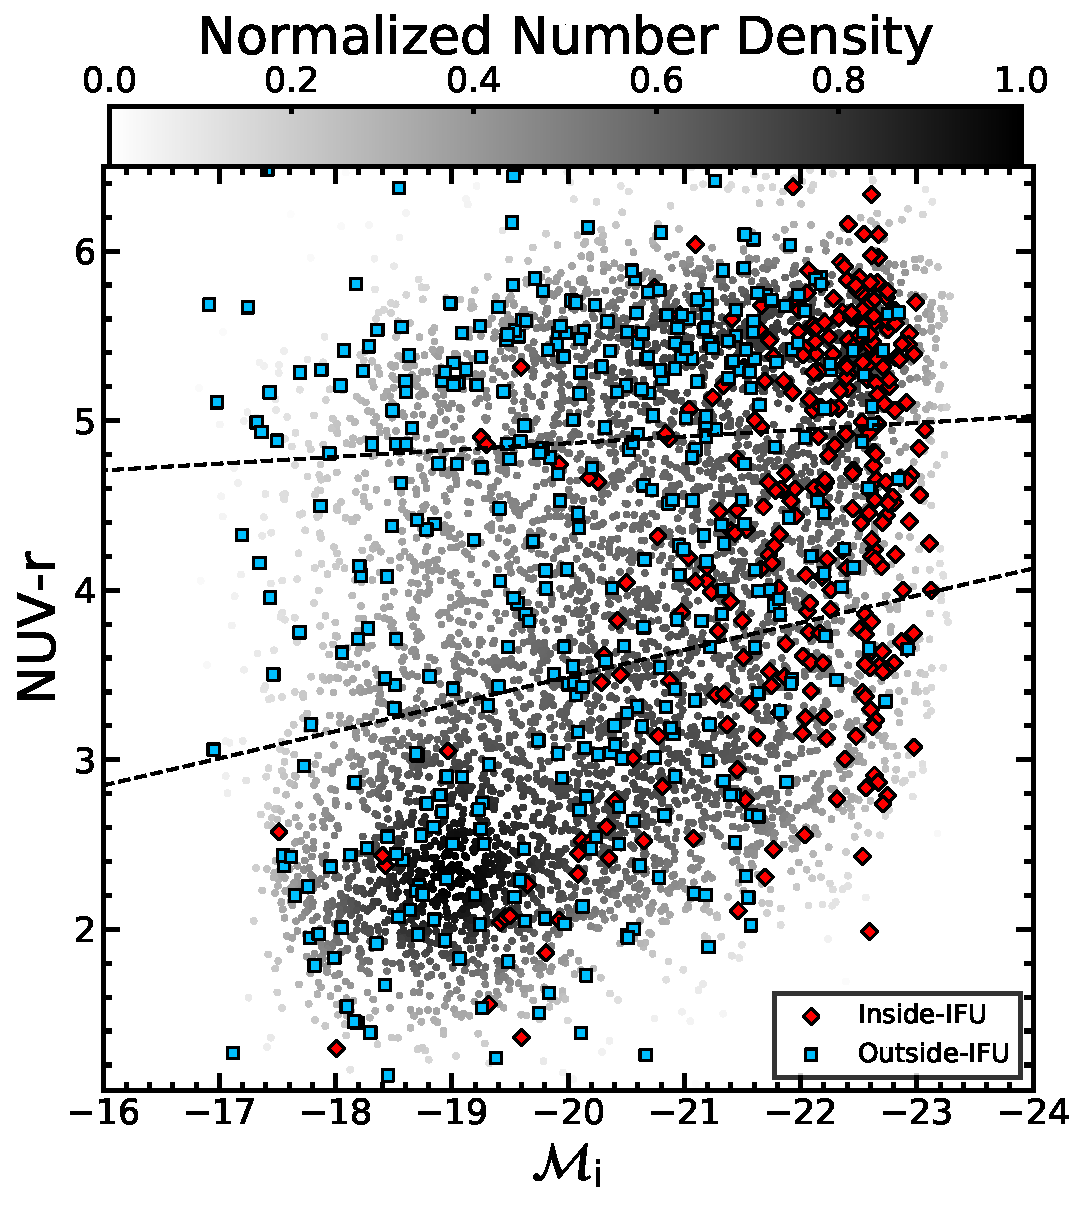
\includegraphics[width=\linewidth]{fig/color-mag.pdf}
\caption[]{Color-magnitude diagram for MaNGA galaxies ({\it colored circles}). The color of the symbol reflects the local density around each data point in this color-magnitude plane, as indicated by the color bar on the top. Inside and outside-IFU pairs are marked with {\it grey diamonds}. From top to bottom, the dashed lines divide the sample into red sequence, green valley, and blue cloud. The star-forming galaxy sample used in this paper are the galaxies below the lower dividing line.}
\label{fig:cmd}
\end{figure}
%%%%%%%%%%%%%%%%%%%%%%%%%%%%%%%%%%%%%%%%%%%%%%

MaNGA is an a IFS survey based at Apache Point Observatory (APO) which used the SDSS (Sloan Digital Sky Survey) 2.5-meter telescope along with two dual-channel BOSS spectrographs \citep{Drory:2015}. MaNGA captures spectra through 17 integral field units (IFUs) with variable numbers of fibers; 19, 37, 61, 91, and 127 fibers covering 12.5\arcsec, 17.5\arcsec, 22.5\arcsec, 27.5\arcsec, and 32.5\arcsec on the sky respectively \citet{Law:2015}. MaNGA is an optical survey with a spectral coverage of 3600$-$10,300 \AA\ with a resolution of R $\sim$ 2000 and a median spectra coverage of 2.5\arcsec\ FWHM \citep{Bundy:2015}. 

The MaNGA survey targets galaxies from a subset of 41,154 galaxies from the NASA-Sloan Atlas (NSA v1\_0\_1; \url{http://www.nsatlas.org}) with a redshift range of 0.01 $<$ z $<$ 0.15 and a luminosity range of -17.7 $<$ $\mathcal{M_{\rm i}}$ $<$ -24.0, where $\mathcal{M_{\rm i}}$ is the rest frame i-band magnitude within the survey's elliptical Petrosian apertures. MaNGA plans to cover 10,000 galaxies with a flat stellar mass distribution at two spatial coverages, 1.5 R/\reff\ and 2.5 R/\reff\ (where \reff\ is the radius which contains 50\% of the galaxy's total light). In this work we use the data from the internal data release, MPL-8, which covers 6142 unique galaxies. 

We classify galaxies in this survey as star forming galaxies using the color-magnitude diagram (CMD). We show the CMD for the MaNGA survey and our pair sample in Figure \ref{fig:cmd} along with demarcation lines which separate the blue cloud, red sequence, and green valley. We established the demarcation lines by collapsing the CMD to a color histogram for each of the three regions. We then varied the slopes between the regions until we found the slopes which best fit the data. These demarcation lines are;

\begin{equation}\label{eq:blue}
NUV-r = 3.1682 - 0.16 (\mathcal{M}_i+18)
\end{equation}
\begin{equation}\label{eq:red}
NUV-r = 4.7866 - 0.04 (\mathcal{M}_i+18)
\end{equation}

Where NUV$-$r is the color and M$_i$ is the i-band magnitude from the NSA catalog. 

After the star formation cuts, we require that all galaxies are in the Primary or Secondary MaNGA subsamples \citep{Wake:2017}. The resulting sample cover a stellar mass range of \logm\ $=$ 9.0$-$11.5.

We build two different pair samples in this work; the inside-IFU sample which contains paired galaxies where both galaxies are covered by a single MaNGA IFU and the outside-IFU sample where a MaNGA target galaxy is coupled with another galaxies found outside of its MaNGA IFU. 

\subsection{Inside-IFU Sample}\label{sec:inside}

In our previous work, \citet{Fu:2018}, using the 2168 unique galaxies form DR14 \citep{Abolfathi:2018} we showed that $\sim$5.7\% of the MaNGA observations have at least one companion galaxy within the field of view of the IFU. In this work we use a refined pair identification process which is also expanded for the most recent internal data release, MPL-8.

We use SDSS photometric objects to create a catalog of objects within the fields of view of the MaNGA IFUs. We extract their spectra from the MaNGA datacubes through a 1\arcsec\ aperture and fit the spectra with {\sc SPFIT} assuming the MaNGA target's redshift. The spectra is then sorted into different categories; ``good" galaxy spectra, broad-line AGN (active galactic nuclei), foreground star, foreground/background galaxies, or poor S/N objects. The ``good" galaxy spectra are the objects whose spectra is well modeled by {\sc SPFIT} at the target galaxy's redshift, whether it is the target galaxy itself or a nearby companion galaxy. This means that the companion galaxy can be within $\pm$3000 km s$^{-1}$ of the MaNGA target. We found 6573 ``good" objects, 57 broad-line AGN, 836 foreground stars, 319 foreground/background galaxies, and 1546 objects with poor S/N. 

From the 6573 galaxies with good spectra, 404 of the MaNGA IFUs have multiple objects within the IFU. We further restrict the sample by setting a relative velocity cut of $\Delta$v $<$ 500 km s$^{-1}$ to remove projected companions and we also require that the galaxies are classified as star forming by the CMD diagram. These requirements reduce our sample down to 124 star forming galaxies (SFGs). 

Several of the target galaxies in our sample have multiple companions. From the whole set of 404 IFUs, there are 327 pairs, 67 triplets, 7 quadruplets, and 1 quintuplet. 

\subsection{Outside-IFU Sample}\label{sec:outside}

We supplement the inside-IFU sample with a set of pairs identified outside of the field of view of the MaNGA IFU. We select these outside-IFU pairs from the NSA catalog. We search for these external pairs by selecting objects with a projected separation from the MaNGA targets of r$_p$ $<$ 50 kpc using the MaNGA target's redshift. We further use a relative velocity cut of $\Delta$v $<$ 500 km s$^{-1}$ to remove projected galaxies from the selection. 

From the NSA catalog's 641,409 galaxies, we find 361 galaxies which are paired to MaNGA targets. MaNGA targets which have both an inside-IFU and an outside-IFU pair are left to the inside-IFU sample. After restricting the sample to SFGs, we have 127 MaNGA targets with paired galaxies outside of the IFU. 

\subsection{Control Sample}\label{sec:control}
We build a sample of isolated control galaxies from the remaining MaNGA galaxies by selecting the MaNGA target galaxies which have no spectroscopic companions within r$_p$ $<$ 50 kpc and $\Delta$v $<$ 500 km s$^{-1}$ either inside or outside of the IFU. This gives us a set of 1891 SFGs and 1528 SFGs which are covered by both \citet{Simard:2011} and \citet{Mendel:2014}. 

The SFR in galaxies has been shown to be dependent on both stellar mass and redshift of the galaxies \citep{Noeske:2007}. This effect needs to be controlled for when comparing the paired and control galaxies to isolate the changes in the sSFR due to merger induced effects. For each galaxy pair we build a subset of 20 control galaxies which are matched in stellar mass and redshift. 

To control for stellar mass, we set a 0.1 dex stellar mass limit between a paired galaxy and the potential control galaxies. To restrict the redshift between the control and paired galaxies, we select control galaxies which are drawn from the same MaNGA subsample (e.g. Primary or Secondary) as the paired galaxy. The MaNGA sample has a tight ``banana" shaped distribution in stellar mass and redshift. By setting a 0.1 dex stellar mass cut and requiring that the galaxies be in the same MaNGA subsample, we effectively set a z $\le$ $\sim$0.025 redshift cut. We note that the MaNGA galaxies with stellar masses above \logm\ $\ge$ 11.0 have a wide redshift distribution, our galaxy samples are restricted to a stellar mass range between \logm\ $=$ 9.0$-$11.0.

Setting the above requirements, most paired galaxies will find between 20$-$100 control galaxies. Since we want each paired galaxy to be treated in a similar manner, we will downselect the total number of acquired control galaxies down to 20 controls using a random number generator. In the cases where a paired galaxy does not initially acquire 20 control galaxies we iteratively expand the stellar mass limit by 0.1 dex until at least 20 control galaxies are found. 

A small set of paired required extra iterations to find 20 controls; 8 paired galaxies need an extra iteration, 1 paired galaxy need two extra iterations, and 1 paired galaxy needed three iterations.

The control galaxies have their radial profiles of sSFR made with both the r-band elliptical Petrosian apertures from the NSA catalog and the r-band elliptical S\'ersic apertures from \citet{Simard:2011}. We use the geometries and stellar masses from \citet{Simard:2011} and \citet{Mendel:2014} when the controls are being matched to pairs in the inside-IFU sample and we use the geometries and stellar masses from the NSA catalog when the controls are being matched to pairs in the outside-IFU sample. 

%%%%%%%%%%%%%%%%%%%%%%%%%%%%%%%%%%%%%%%%%%%%%%%%%%%%
\section{Radial Profiles of Star Formation}\label{sec:analysis}

%%%%%%%%%%%%%%%%%%%%%%%%%%%%%%%%%%%%%%%%%%%%%%
%\begin{figure}
%\centering
%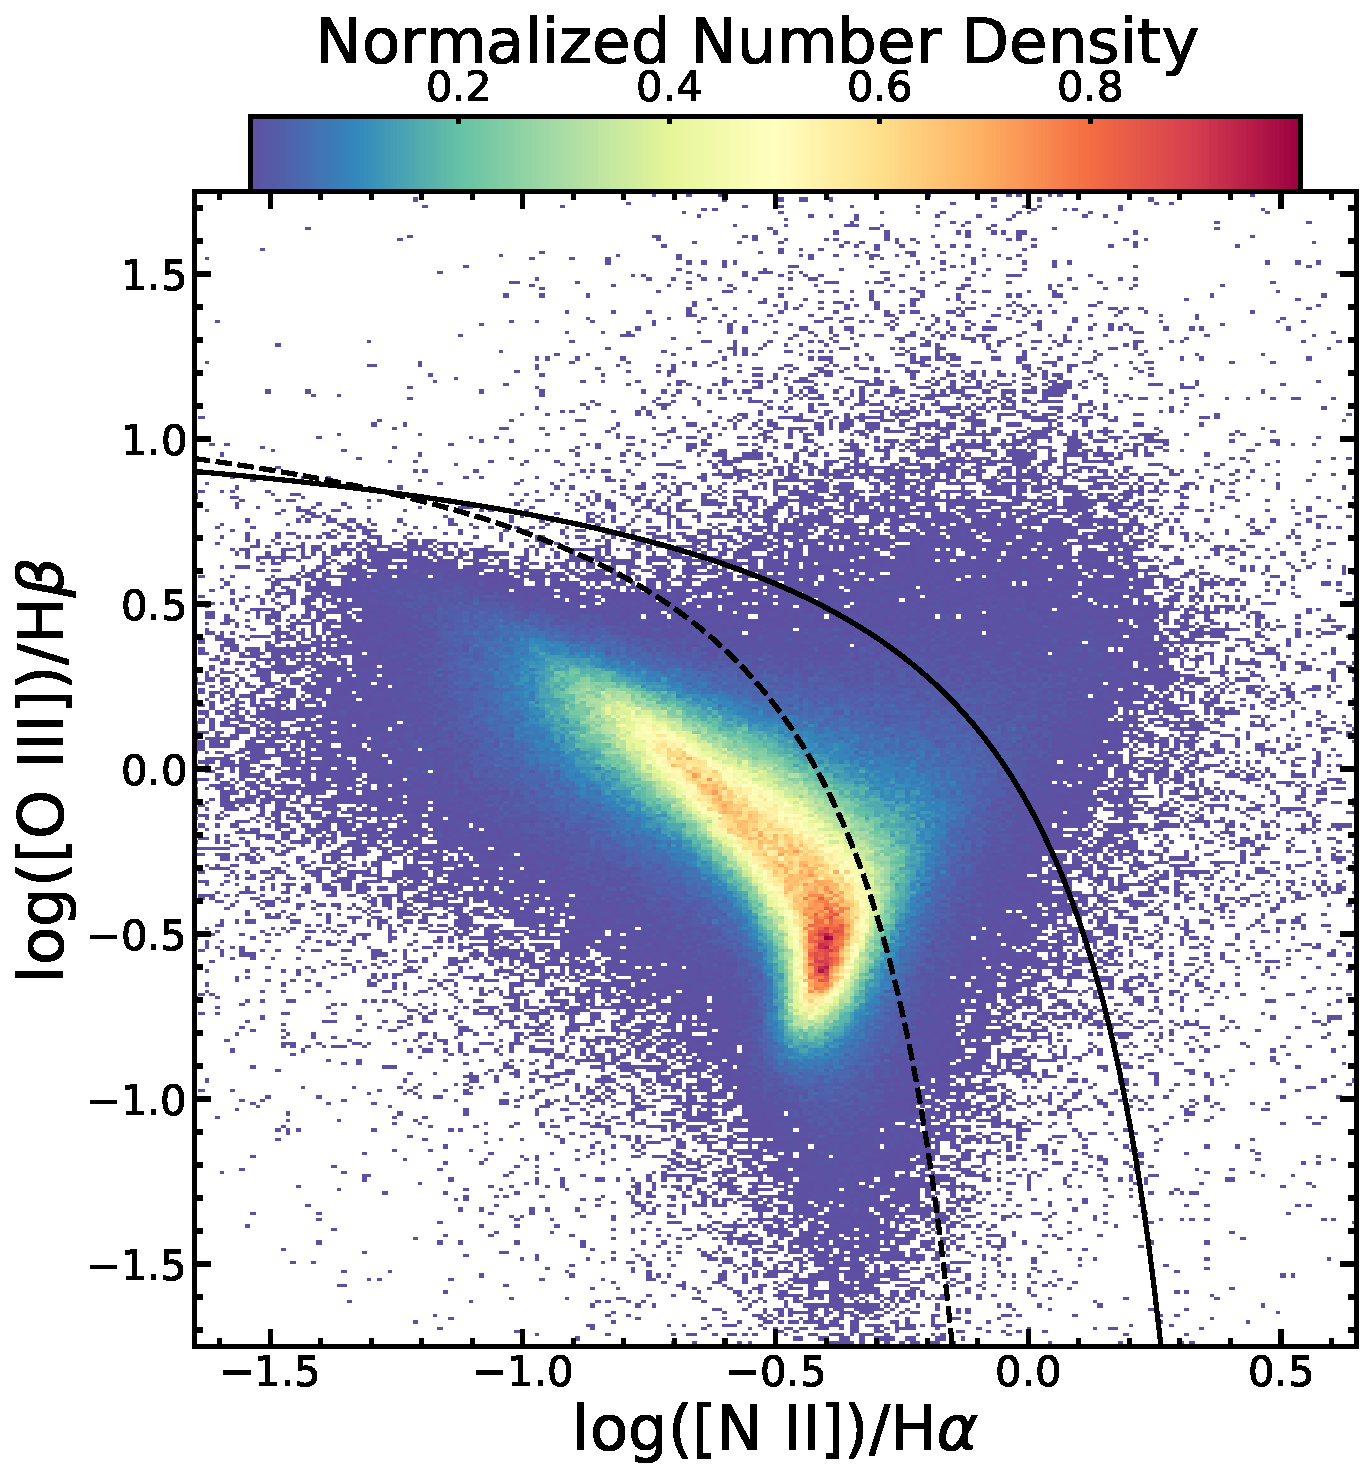
\includegraphics[width=\linewidth]{fig/bpt_spax.pdf}
%\caption[]{The 2-D histogram showing the BPT classification \citep{Baldwin:1981} of individual spaxels within our star-forming control and pair samples. The color of each bin represents the number density of spaxels, normalized to one. The solid black line represents the theoretically determined maximum starburst line of \citet{Kewley:2001} and the dashed black line is the analytical \citet{Kauffmann:2003} line.}
%\label{fig:bpt}
%\end{figure}
%%%%%%%%%%%%%%%%%%%%%%%%%%%%%%%%%%%%%%%%%%%%%%

\subsection{Emission Line Extraction}

%%% SPFIT
We use our own {\sc IDL} based spectral fitting code, {\sc SPFIT}, to model the spectra from the MaNGA datacubes. {\sc SPFIT} simultaneously fits emission lines and the stellar continuum with the Levenberg-Marquardt nonlinear least-squares minimization algorithm \citep{Fu:2018}. Emission lines are parameterized as a Gauss-Hermite series and the stellar continuum is the sum of simple stellar populations (SSPs) convolved with the line-of-sight velocity distribution (LOSVD). The algorithm provides us with measurements of emission line fluxes, equivalent widths, velocities, and velocity dispersions of 19 emission lines and measurements of stellar masses, ages, [Fe/H], and the kinematics of the stellar populations. 

%%% Reddening
We correct the emission lines for reddening using the extinction curve from \citet{Cardelli:1989} with updated coefficients from \citet{ODonnell:1994}. The extinction in parameterized as R$_V$ $\equiv$ A$_V$/E(B$-$V) $=$ 3.1, where we estimate the value of the V-band extinction, A$_V$, by comparing the H$\alpha$/H$\beta$ ratio to the expected value of 2.85 for case-B recombination. The extinction correction is applied to all of the extracted emission lines.

\subsection{Star Formation Rate}

We measure the SFR from the H$\alpha$ luminosity, L$_{H\alpha}$, calculated from the H$\alpha$ flux.  We use the SFR formula, Equation \ref{eq:sfr}, from \citet{Murphy:2011} which uses a Kroupa IMF, Solar metallicity, a constant SFR at an age of 100 Myr, and Case-B recombination. 

\begin{equation}\label{eq:sfr}
\frac{\rm{SFR}}{M_{\odot} \, \rm{yr^{-1}}} = \frac{L_{H\alpha}}{1.86 \times 10^{41}\, \rm{erg\,s}^{-1}}
\end{equation}

Since the stellar mass of a galaxy is not uniformly distributed within the galaxy, we normalize the SFR by the local stellar mass, giving us the specific star formation rate (sSFR). The local stellar masses used here is the stellar mass calculated by {\sc SPFIT}'s fit to the stellar continuum within each spaxel (spatial pixel).

\begin{equation}
{\rm sSFR} = \frac{\rm SFR}{M^*}
\end{equation}

This will allow us to compare the SFR in high mass regions, like the centers of the galaxies, to the SFR lower mass regions, like the disk of the galaxies.


We use the BPT diagnostic \citep{Baldwin:1981} to remove spaxels which were not ionized by star formation. To separate ionization sources, we use the theoretical maximum starburst line from \citet{Kewley:2001} (Equation \ref{eq:kewley}).

\begin{equation}\label{eq:kewley}
\rm{log\Big(\frac{[O\,\textsc{iii}]\lambda 5007}{H\beta}\Big) = \frac{0.61}{log([N\,\textsc{ii}]\lambda 6584 / H\alpha) - 0.47} + 1.19}
\end{equation}

Where \OIII$\lambda$5007, H$\beta$, \NII$\lambda$6584, and H$\alpha$ are emission line fluxes within each MaNGA spaxel. We use the \citet{Kewley:2001} demarcation line as the limit for classifying star formation in the MaNGA spaxels. 

It has also been shown that hot low mass evolved stars (HOLMES) in retired galaxies can mimic HII regions and AGN on the BPT diagram \citep{Stasinska:2008}. We apply an H$\alpha$ equivalent width (EW) cut of \ewha\ $>$ 3\AA\ to mask retired spaxels \citet{Cid-Fernandes:2011}. 

 

%%%%%%%%%%%%%%%%%%%%%%%%%%%%%%%%%%%%%%%%%%%%%%%%%%%%
\subsection{Geometry}\label{sec:radial}

%%%%%%%%%%%%%%%%%%%%%%%%%%%%%%%%%%%%%%%%%%%%%%
\begin{figure*}
\centering
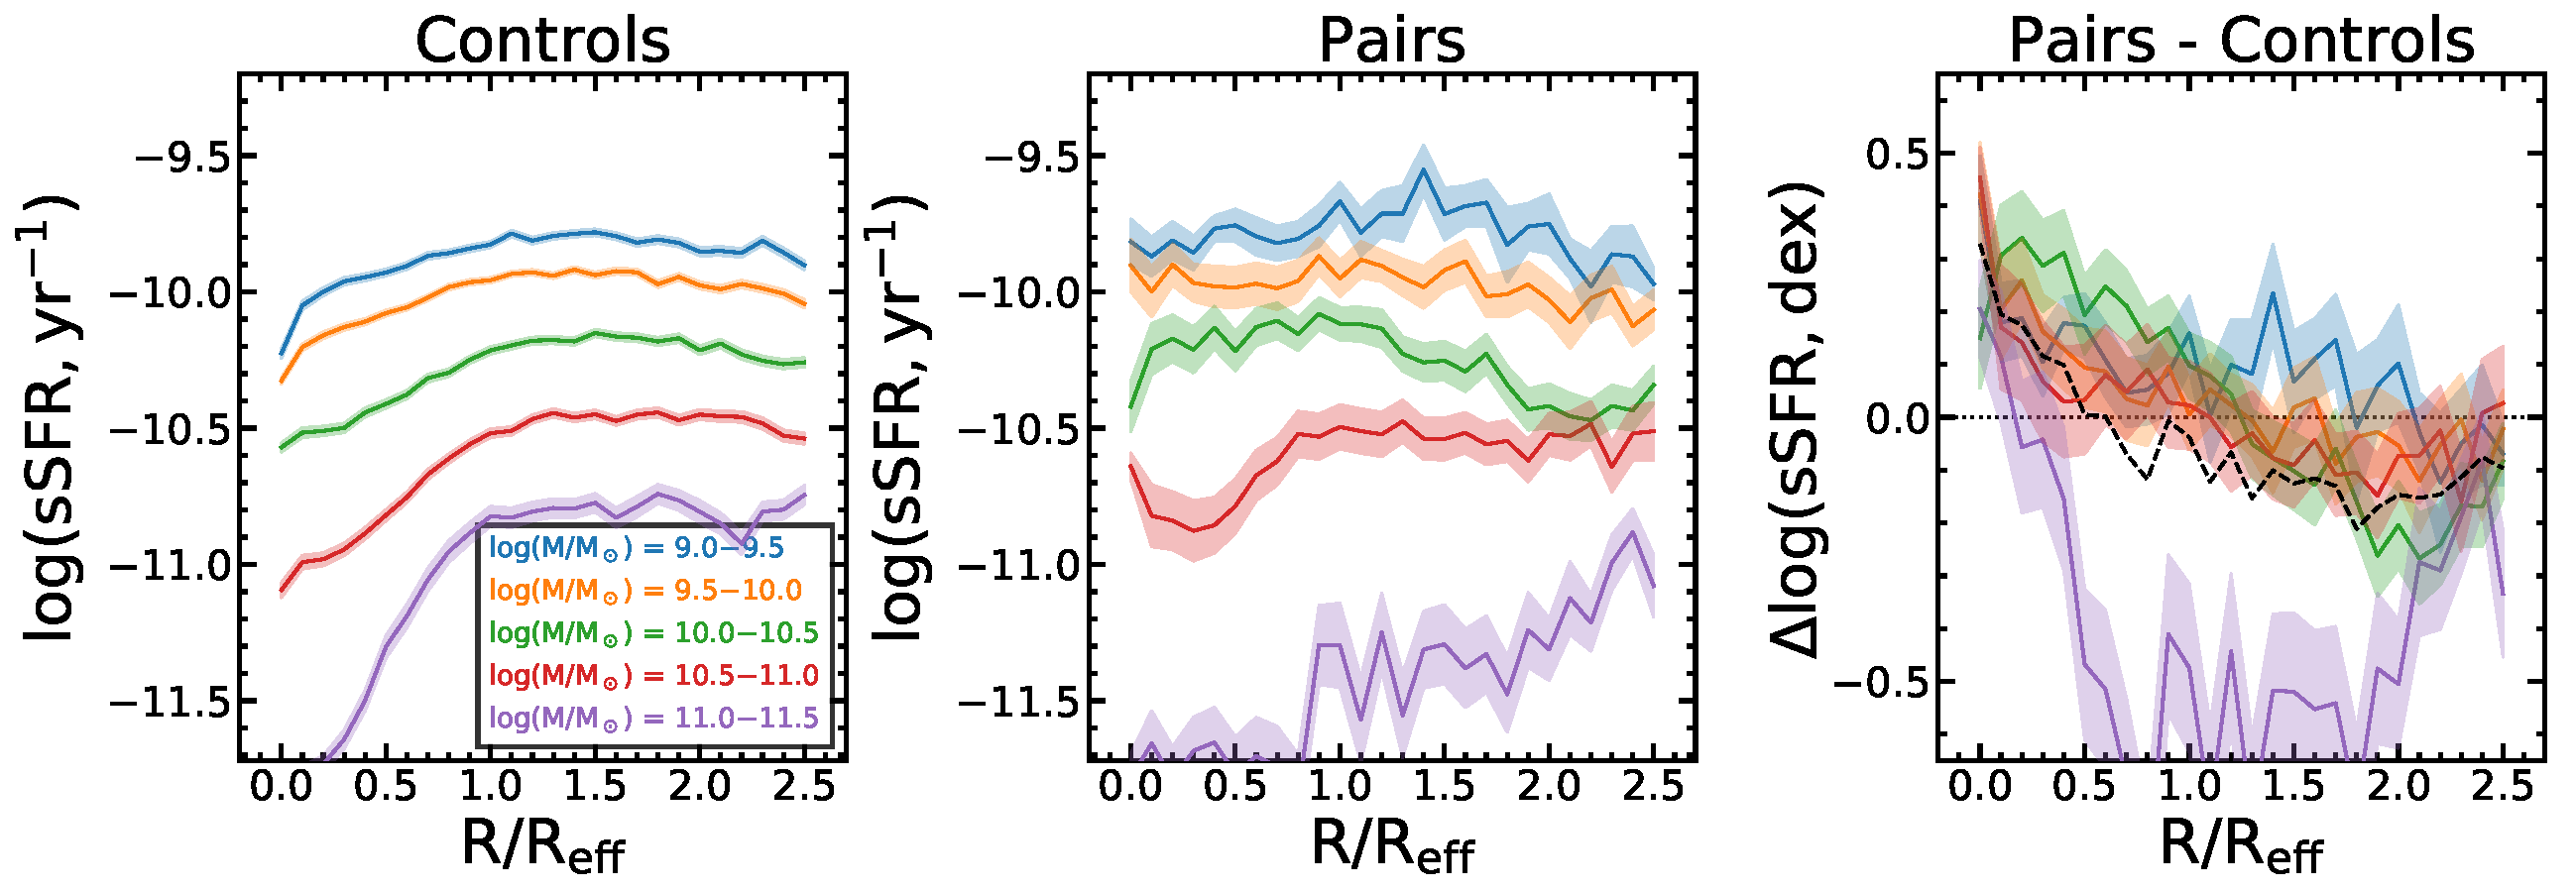
\includegraphics[width=\linewidth]{fig/ssfr_comb.pdf}
\caption[]{The log(sSFR) as a function of galactocentric radius for control galaxies (\textbf{Left}) and galaxy pairs (\textbf{Middle}). The difference between the profiles of the paired galaxies and the control galaxies are shown in the \textbf{Right} panel. The dashed black profile represents the mean of the difference profiles). The colors of the profiles represent the mass range of the selected galaxies and the highlighted region around the profiles represent the standard error of the mean of the data at the given radius interval.}
\label{fig:ssfr_prof}
\end{figure*}
%%%%%%%%%%%%%%%%%%%%%%%%%%%%%%%%%%%%%%%%%%%%%%

We characterize the geometry of the inside-IFU galaxies with the r-band elliptical S\'ersic apertures from \citet{Simard:2011} and we characterize the total stellar mass of the galaxies with the stellar masses from \citet{Mendel:2014}. We use \citet{Simard:2011} instead of the apertures from the NSA catalog, which the MaNGA sample is drawn from, because the apertures in the NSA catalog often fail to fit the MaNGA galaxies when there is another nearby, bright object. 

The \citet{Simard:2011} and \citet{Mendel:2014} catalogs do not completely cover the MaNGA sample. Out of the 124 SFGs in the inside-IFU sample, 33 of the SFGs are covered by both \citet{Simard:2011} and \citet{Mendel:2014}.

We use the r-band elliptical Petrosian apertures from the NSA catalog to describe the geometry of the galaxies in the outside-IFU sample. For cases where the identified galaxy pair is outside of the MaNGA IFU, the NSA catalog's algorithm is able to fit the MaNGA target's geometry well. We also use the stellar masses calculated from the r-band elliptical Petrosian apertures in the NSA catalog for the total stellar mass of the galaxies. \\


In order to spatially characterize the star formation in the paired galaxies we build radial profiles of sSFR. As mentioned in Section \ref{sec:data} we use the r-band elliptical Petrosian apertures from the NSA catalog and the r-band S\'ersic apertures from \citet{Simard:2011} to define the geometries of the galaxies. We calculate the inclination angle, {\it i}, of the galaxies using the major-to-minor axis ratios from the elliptical apertures;

\begin{equation}
{\rm cos^2}(i) = \frac{(b/a)^2 - q^2}{1 - q^2}
\end{equation}

Where $q$ is the intrinsic oblateness. We use the empirically determined oblateness of $q = 0.13$, from \citet{Giovanelli:1994}.

The inclination angle, along with the galaxy's position angle, is used to deproject the geometries of the galaxies. The distance to each of the spaxels from the center of the MaNGA target is calculated using the 50\% half light radius to scale the size of the galaxy. The r-band elliptical S\'ersic apertures from \citet{Simard:2011} are used for the inside-IFU sample and their controls and the r-band elliptical Petrosian apertures from the NSA catalog are used for the outside-IFU sample and their controls. 

The spaxels are binned into radius increments of 0.1 R/\reff\ from 0.0$-$2.5 R/\reff. Within each radius bin we take the median of the specific star formation rate. The profiles' errors are the standard error of the mean of the data within each radius bin. We create one of these individual averaged radial profiles for every MaNGA galaxy. 

We use our catalog of photometric objects and the \citet{Simard:2011} catalog to mask foregournd/background objects which may contaminate the data. Objects in our photometric catalog are masked out with a 2\arcsec\ circular aperture and the galaxies from \citet{Simard:2011} are masked out with a 2.0 R/\reff\ elliptical aperture, using the r-band S\'ersic apertures from the catalog. 

With individual log(sSFR) profiles built for each MaNGA galaxy, we now use two different methods to compare the profiles of paired galaxies against the profiles of control galaxies. The first method, in Section \ref{sec:mass-bin}, paired galaxies are compared to control galaxies within evenly spaced stellar mass-bins. In the second method, in Section \ref{sec:tailored}, paired galaxies are compared to a subset 20 control galaxies which have a similar stellar mass and redshift. 

%%%%%%%%%%%%%%%%%%%%%%%%%%%%%%%%%%%%%%%%%%%%%%%%%%%%
\section{Results}\label{sec:results}

\subsection{Mass-Binned Difference Profiles}\label{sec:mass-bin}

In the first method, paired and control galaxies are grouped into four evenly spaced stellar mass bins between \logm\ $=$ 9.0$-$11.0. Within each stellar mass bin, we create a median profile of log(sSFR) as a function of galactocentric radius for both paired and control galaxies. The control profiles are constructed using all available control galaxies within each mass bin. The error associated with the profile is the standard error of mean of the data at each radius bin. We show these ``stacked" profiles for control galaxies in the left hand panel of Figure \ref{fig:ssfr_prof} and the stacked profiles for paired galaxies in the middle panel of Figure \ref{fig:ssfr_prof}.

Once the stacked profiles are made, we take the difference between the stacked profiles of the paired galaxies and the control galaxies, pair - control, in log space (this means that the profiles really represents a ratio between the pairs and controls in linear space). This gives us difference profile, $\Delta$log(sSFR), which shows us where the sSFR is enhanced or suppressed (shown in the right hand panel of Figure \ref{fig:ssfr_prof}). We will discuss the results of the difference profiles later in Section \ref{sec:results}.

\subsection{Tailored-Controls Difference Profiles}\label{sec:tailored}

In the second method, we match each paired galaxy to a set of 20 control galaxies of a similar stellar mass and redshift, as mentioned in Section \ref{sec:control}. We take the individual averaged profiles of the selected control galaxies and take the median value of the profiles at each radius bin giving us a stacked profile of control galaxies. The error of the profile is the standard error of the mean of the individual profiles. We also take into account the error associated with the random selection of controls using a bootstrapping method to quantify the variation in the values of the stacked profiles over 1000 iterations. This random selection contributes an error of about 0.1 dex.

Once the stacked profile of the control galaxies is made, we take the difference between the paired galaxy's profile and the stacked control profile in log space. We do this process for each of the 160 paired galaxies. 

The difference profiles at this stage have now been controlled for stellar mass, redshift, and galaxy size. We can freely stack these profiles to study the global properties of the merging galaxies. We take all of the $\Delta$log(sSFR) profiles and take the median value within each radius bin to create a stacked profile of the individual difference profiles. We split the individual difference profiles into four evenly spaced stellar mass bins between \logm\ $=$ 9.0$-$11.0 and stack the difference profiles within each mass bin. This gives us four difference profiles covering four different stellar mass ranges shown in the left hand panel of Figure \ref{fig:ssfr_mass}. The results of the profiles will discussed in detail in Section \ref{sec:results}.

To study how the star formation in the centers of paired galaxies are affected by merger events, we extract the $\Delta$log(sSFR) from the individual difference profiles. We extract the value of $\Delta$log(sSFR) from the inner 0.5 R/\reff\ of the paired galaxies and take the mean value of the $\Delta$log(sSFR) within the aperture. We depict the central $\Delta$log(sSFR) as a function of stellar mass in the right hand panel of Figure \ref{fig:ssfr_mass}.

%%%%%%%%%%%%%%%%%%%%%%%%%%%%%%%%%%%%%%%%%%%%%%
\begin{figure*}
\centering
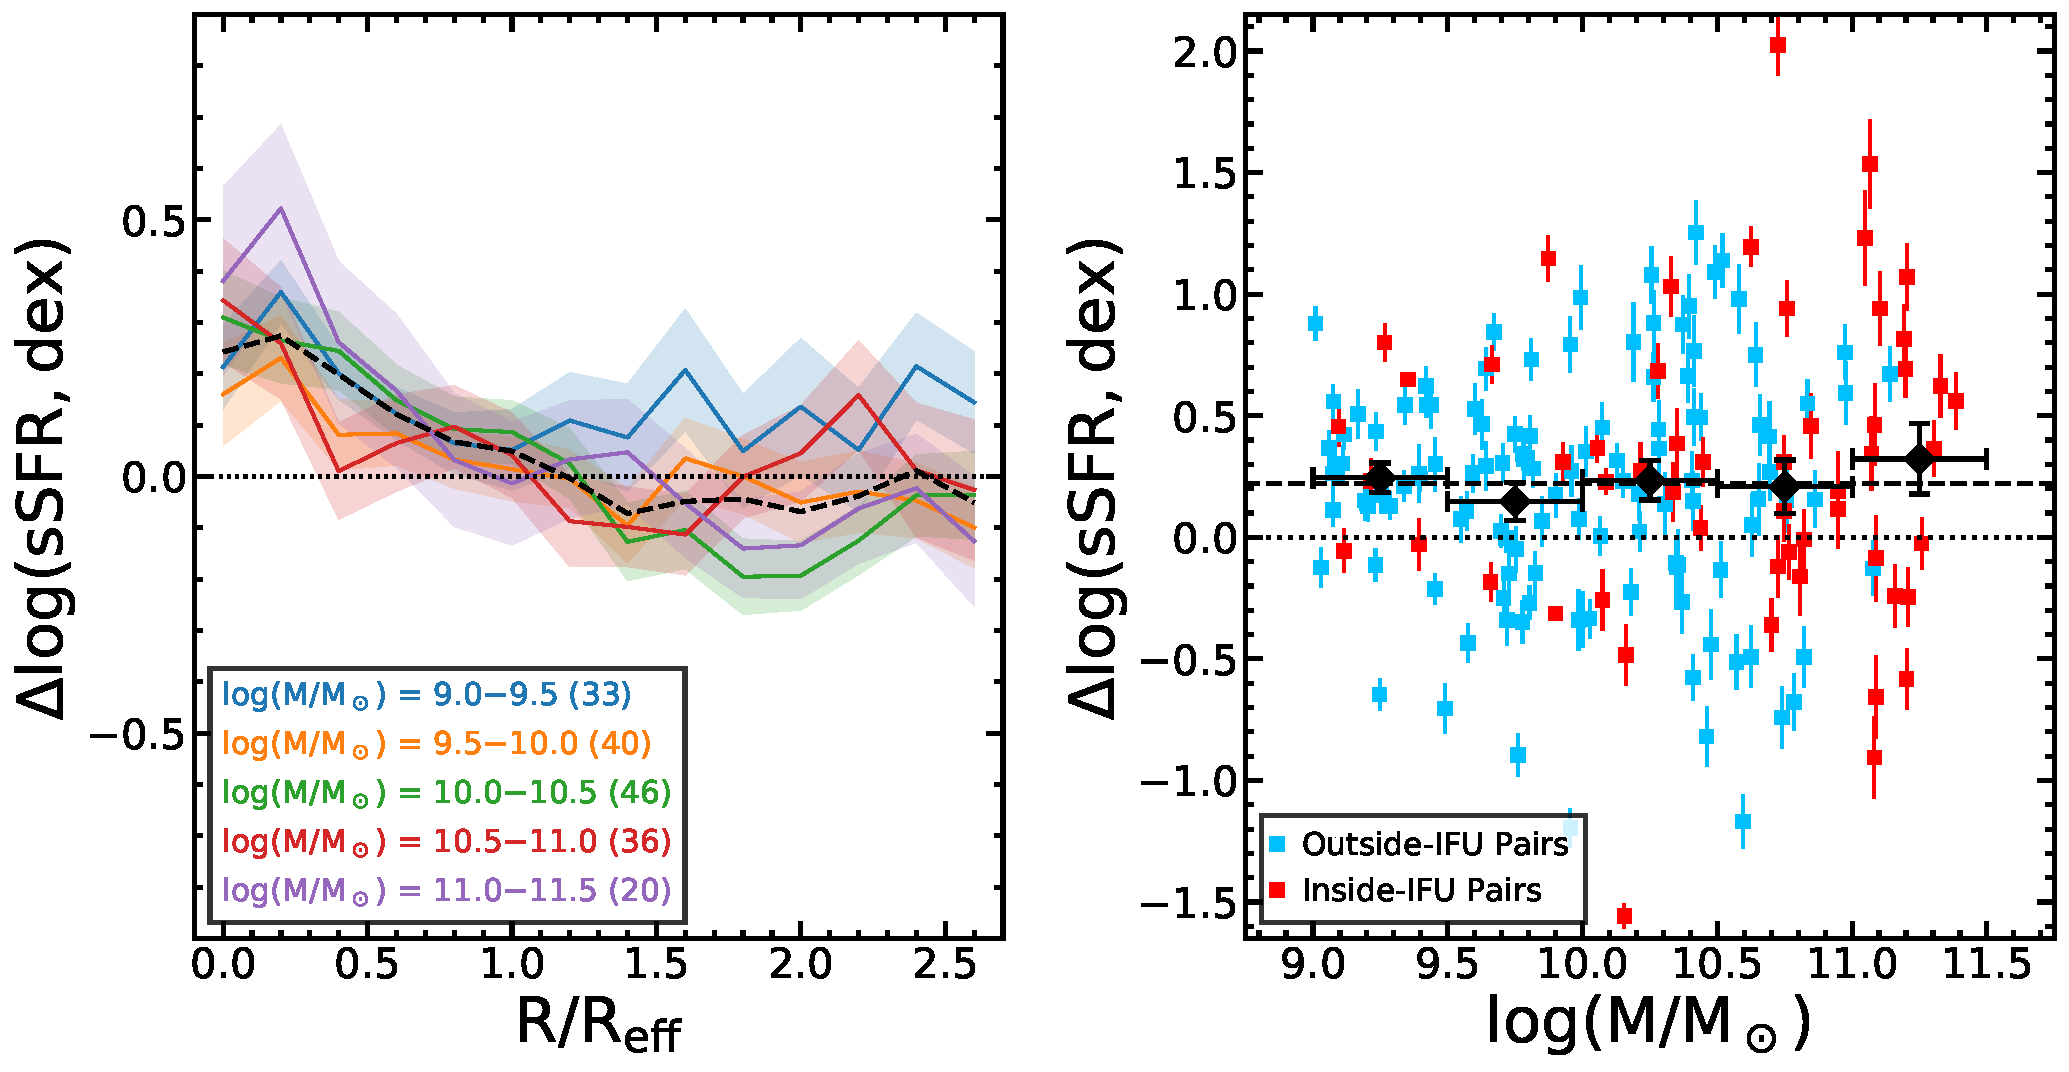
\includegraphics[width=\linewidth]{fig/ssfr_mass.pdf}
\caption[]{The \textbf{Left} panel shows the $\Delta$log(sSFR) profiles where the difference profiles are constructed from the difference between the paired galaxy profiles and a set of 20 control galaxies. The profiles are split into four different stellar mass bins and the highlighted region about the profiles represent the standard error of mean of the profile. The black dashed line represents the mean profile between the four difference mass ranges. In the \textbf{Right} panel the nuclear $\Delta$log(sSFR) are shown. The black squares are the mean values within a stellar mass bin (where the size of the bins are shown the the horizontal error bars). The vertical error bars on the black squares represent the standard deviation within the bin. The horizontal, dashed black line represents the median central enhancement of the pair sample. Galaxies in the outside-IFU (Blue) and inside-IFU (Red) samples are separately depicted.}
\label{fig:ssfr_mass}
\end{figure*}
%%%%%%%%%%%%%%%%%%%%%%%%%%%%%%%%%%%%%%%%%%%%%%

\subsection{Stellar Mass}

In Figures \ref{fig:ssfr_prof} and \ref{fig:ssfr_mass}, we show the profile of $\Delta$log(sSFR) as a function of galactocentric radius between two different methods of comparing paired galaxies to control galaxies. In the first method (Section \ref{sec:mass-bin}) where pair and control galaxies are compared within different stellar mass bins. The difference profiles from this method show a central enhancement to the log(sSFR) of $\sim$0.3 $\pm$ 0.1 dex. The enhancement linearly falls to zero at 1.0 R/\reff\ after which the disks of the paired galaxies have zero enhancement/suppression to their sSFR. 

The $\Delta$log(sSFR) profile following the second method shows the same central sSFR enhancement albeit with smaller variances. Within the inner 1.0 R/\reff, there is a variance between the profile of 0.1 dex. Beyond 1.0 R/\reff, the variance increases 0.2 dex. This indicates that the second method of pair$-$ control comparison is superior to the first method. 

The profiles of either method show no dependence on the stellar mass of the galaxies.  This effect is better seen in the right hand panel of Figure \ref{fig:ssfr_mass} where the nuclear $\Delta$log(sSFR) of the paired galaxies fall within 0.1 dex of the mean nuclear sSFR enhancement. Low mass galaxies have their star formation enhanced at the same level as high mass galaxies. The similar level of $\Delta$log(sSFR) in high and low mass galaxies will mean that the fractional mass growth between high and low mass galaxies will be different.

\subsection{Future Mass Growth}

The higher rate of star formation within interacting galaxies will mean that the stellar mass in the interacting galaxies will grow at a faster rate compared to secular mass growth. The question is whether or not the advanced mass growth rate is significant. 

To estimate the enhanced mass growth rate due to merger induced star formation, we will assume a constant star formation rate over a given dynamic timescale, $\tau_{dyn}$. A specific star formation rate is already a representation of the fractional mass growth every year, so the merger induced mass growth is simply;

\begin{equation}
\frac{\Delta M_{merger}}{M_{total}} = \left(sSFR_{pair} - sSFR_{control}\right) * \tau_{dyn}
\end{equation}

For this estimation we use a timescale of 1 Gyr, which is the order of the typical timescale between the passage of the first and second pericenters in hydrodynamical simulations \citep{Boylan-Kolchin:2008}. 

To get the difference in sSFR between the pairs and controls, we fit a gaussian to the difference profiles split by stellar mass. We then add the modeled difference profile to the stacked control profile in the same mass range in log space. We then take the difference between the profiles in linear space and multiply the difference by the 1 Gyr timescale. 

We show the mass growth rate profile for each of the four mass ranges in Figure \ref{fig:mass_gain_sum}. The mass growth rate is largely restricted to the centers of the galaxies and falls to zero around 1.0 R/\reff, following profile of the $\Delta$log(sSFR). The mass growth rate is strongly dependent on the stellar mass of the paired galaxies. 

The fractional mass change is greatest in the less massive galaxies, $\Delta$M$_{merger}$/M$_{total}$ $=$ 0.065, while it is less substantial is the more massive galaxies, $\Delta$M$_{merger}$/M$_{total}$ $=$ 0.015. This is unsurprising as the $\Delta$log(sSFR) profiles were independent of the galaxies' total stellar mass. 

Galaxies in the mass range \logm\ $=$ 9.0$-$10.0 have a mass growth of $\sim$1.6$\times$ that of secular mass growth and galaxies in the mass range \logm\ $=$ 10.0$-$11.0 have a mass growth of $\sim$2.3$\times$ that of secular mass growth. While low mass galaxies may see a more substantial change to their total stellar mass, the more massive galaxies experience higher growth rates.

In the context of galaxy evolution, where less massive galaxies merge to form larger galaxies, the merger induced star formation contributes a significant amount of stellar mass on top of the stellar mass contribution from the mixing of the two galaxies. Further, the merger induced mass growth is restricted to the centers of the paired galaxies which will result in galaxies which have more prominent bulges in their centers.  

%%%%%%%%%%%%%%%%%%%%%%%%%%%%%%%%%%%%%%%%%%%%%%%%%%%%
\section{Discussion}\label{sec:disc}
%%%%%%%%%%%%%%%%%%%%%%%%%%%%%%%%%%%%%%%%%%%%%%
\begin{figure}
\centering
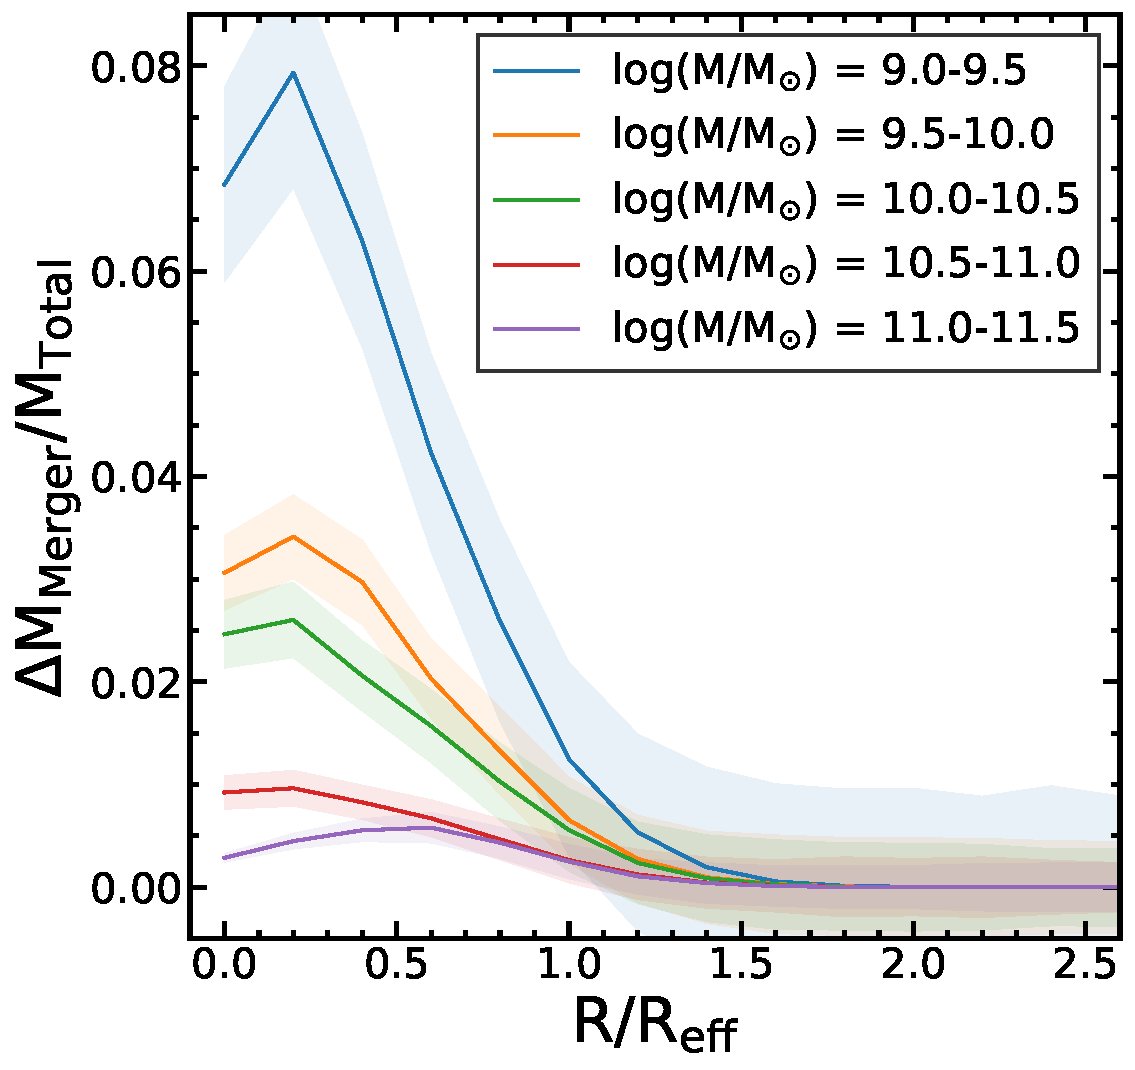
\includegraphics[width=3in]{fig/mass_gain.pdf}
\caption[The fractional mass gain due to merger induced star formation.]{The fractional mass growth due to merger induced star formation over a dynamical timescale, $\tau$ $=$ 1 Gyr. The highlighted region represents the propagated standard errors of the mean of the stacked log(sSFR) profiles. }
\label{fig:mass_gain_sum}
\end{figure}
%%%%%%%%%%%%%%%%%%%%%%%%%%%%%%%%%%%%%%%%%%%%%%

%%%%%%%%%%%%%%%%%%%%%%%%%%%%%%%%%%%%%%%%%%%%%%
\begin{figure*}
\centering
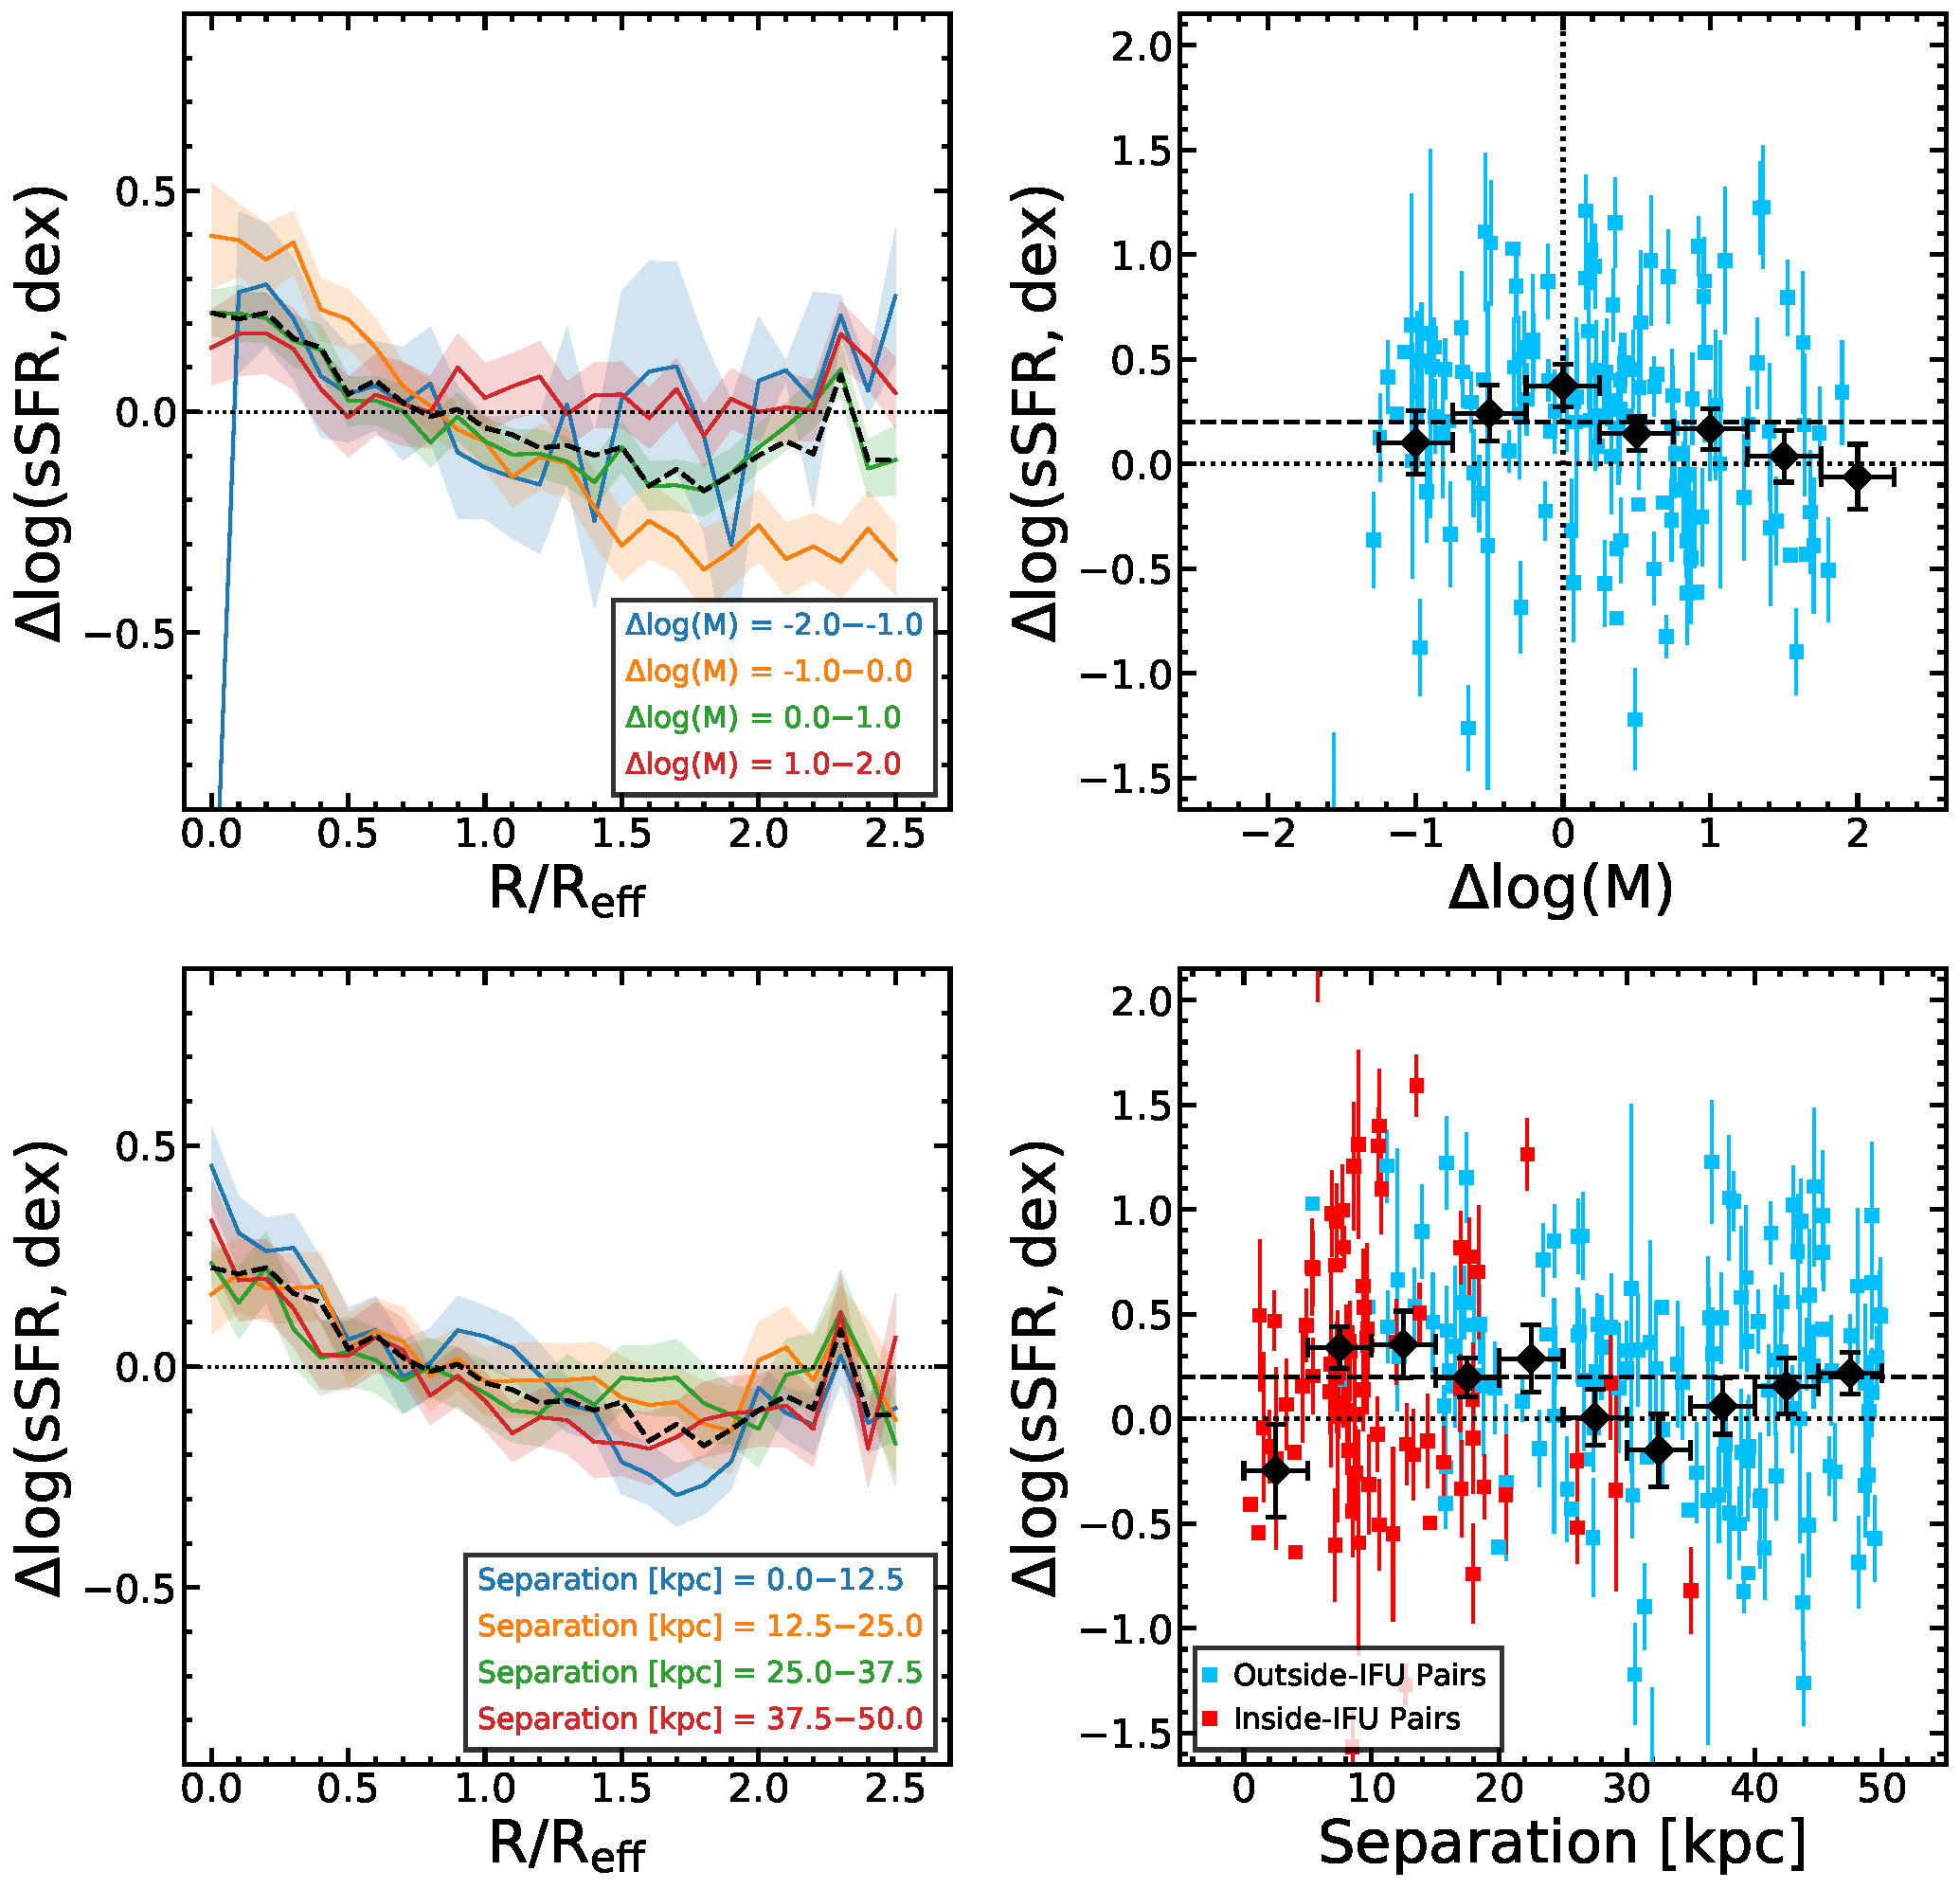
\includegraphics[width=\linewidth]{fig/ssfr_partial.pdf}
\caption[]{Same as Figure \ref{fig:ssfr_mass} except the difference profiles are split by mass ratio (\textbf{Top row}) and projected separation (\textbf{Bottom row}). }
\label{fig:ssfr_dmsep}
\end{figure*}
%%%%%%%%%%%%%%%%%%%%%%%%%%%%%%%%%%%%%%%%%%%%%%

In this work, we primarily focused on how the $\Delta$log(sSFR) in paired galaxies behaves as a function of stellar mass. We also explored how the $\Delta$log(sSFR) behaves as a function of the mass ratio between the paired galaxies and the projected separation between the paired galaxies. While we see hints that the $\Delta$log(sSFR) is affected by the mass ratio and projected separation, these results are less definitive than the $\Delta$log(sSFR) profile's lack of dependence on stellar mass. 


\subsection{Mass Ratio}
While the total stellar mass between the galaxies has no effect on the merger induced star formation, the mass ratio between the paired galaxies does. The mass ratio here is calculated as the difference between stellar masses contained within the 50\% half light radius, 

\begin{equation}
\Delta {\rm log}(M) = {\rm log}(M_{target}) - {\rm log}(M_{comp}) 
\end{equation}

Where M$_{target}$ is the stellar mass of the MaNGA target galaxy and M$_{comp}$ is the stellar mass of the companion galaxy. Note that we do not use the absolute value of the difference like how the mass ratio is typically used. We do this so that we can independently study how the star formation large central galaxies behave in comparison to small satellite galaxies.

For the outside-IFU sample we use the stellar masses calculated from the r-band elliptical Petrosian apertures from the NSA catalog. For the inside-IFU sample, neither the NSA catalog nor \citet{Mendel:2014} will cover both galaxies. Instead we use stellar masses calculated from {\sc SPFIT} from the inner 2\arcsec\ of the galaxies. 

In the Top row of Figure \ref{fig:ssfr_dmsep} we see that the sSFR enhancement is strongest in galaxies close to a 1:1 mass ratio, $\Delta$log(M) $=$ 0.0. These galaxies feature a central enhancement of $\sim$0.4 dex which is 0.15 dex higher than the average central enhancement of the whole sample. This enhancement falls with wider mass ratio; however, pairs with large differences in stellar mass still feature substantial levels of star formation enhancement, 0.2$-$0.25 dex at mass ratios of $|\Delta$log(M)$|$ $=$ 1.0.

We also use the mass ratio to explore how the merger induced tidal torques affect paired galaxies with large mass ratios, $|\Delta$log(M)$|$ > 0.5. We use the mass ratio to separate the massive central galaxy from satellite galaxies. A paired galaxy with a positive mass ratio is the more massive galaxy of the pair while a paired galaxy with negative mass ratio is the less massive galaxy. We see that the less massive galaxy of a pair show a higher level of sSFR enhancement, by $\sim$0.1 dex, with respect to the more massive galaxy. This shows us that satellite galaxies may be more susceptible to tidal interactions than the central galaxies in the pair system. 

In previous studies it was noted that the enhancement to the SFR is strongest in galaxy pairs with small mass ratios \citet{Ellison:2008}. We see the same effect; however, we have also shown that galaxy pairs with large mass ratios still show a substantial level of sSFR enhancement. It has been a convention to split galaxy pairs in major mergers, $|$log(M)$|$ $\le$ 0.5, and minor mergers 0.5 $<$ $|$log(M)$|$ $\le$ 1.0. In this work, we can see that the mass ratio range used in galaxy pair studies could be widened to at least $|$log(M)$|$ $\le$ 2.0 so that larger pair samples can be constructed.  

Further, within these galaxy pairs with wide mass ratios we see that the less massive galaxy in the pair shows higher levels of sSFR enhancement. This implies that satellite galaxies are more affected by interaction induced star formation than the central galaxy. 

\subsection{Projected Separation}\label{sec:sep}

We also look at the level of sSFR enhancement as a function of the projected separation between the two galaxies in the bottom row of Figure \ref{fig:ssfr_dmsep}. The $\Delta$log(sSFR) profiles show a clear gradient with the projected separation where close galaxy pairs show higher levels of sSFR enhancement compared to pairs with wide separations. The profiles in the galaxy pairs in the separation range, r$_p$ $=$ 0.0$-$12.5, are $\sim$0.1 dex above the median and the the profiles of the galaxy pairs in the separation range, r$_p$ $=$ 37.5$-$50.0, are $\sim$0.1 dex below the median. 

This effect can be seen most clearly in the scatter plot of the central $\Delta$log(sSFR) enhancement as a function of projected separation. The level of the enhancement gradually increases with closer separation from 50 kpc to 10 kpc. While $\Delta$log(sSFR) falls at higher separations, there is still a substantial level of enhancement between 40 and 50 kpc, $\sim$0.1$-$0.2 dex. Within 15 kpc, the $\Delta$log(sSFR) enhancement jumps to 0.5$-$0.6 dex. 

The sSFR enhancement increasing with closer projected separations is to be expected and has been shown in previous studies \citep{Ellison:2008, Scudder:2012, Patton:2013}. The passage of the first pericenter is predicted to trigger a burst of star formation which falls as the two galaxies separate \citep{Scudder:2012}. The sSFR enhancement in our sample persists out to 50 kpc, \citet{Patton:2013} showed that the burst of star formation can persist out to 150 kpc. 

For the galaxies with the closest separations, r$_p$ $<$ 5 kpc, $\Delta$log(sSFR) drops to zero. This is strange as we would expect that the closest pairs would show the strongest enhancements to their star formation as they are currently or have just passed the first pericenter. This seems odd as one would think that these galaxies should show the strongest enhancements to the sSFR. 

This lack of $\Delta$log(sSFR) could be due to a couple of reasons. First, it may be due to the limited sampling of this separation range, there are only 6 paired galaxies in this range. A second explanation could be that we are observing merging galaxies which are just going though their first pericenter, but have yet to have the burst of star formation. Not enough time has elapsed for the gas inflows from the disks of the galaxies to reach the centers of the galaxies. The hydrodynamical simulations of \citet{Scudder:2012} show this delay in the burst of star formation, where the burst of star formation only reaches its peak after 0.3 Gyr after the passage of the first pericenter. 

\subsection{Comparison with Previous Works}

%%%%%%%%%%%%%%%%%%%%%%%%%%%%%%%%%%%%%%%%%%%%%%
\begin{figure}
\centering
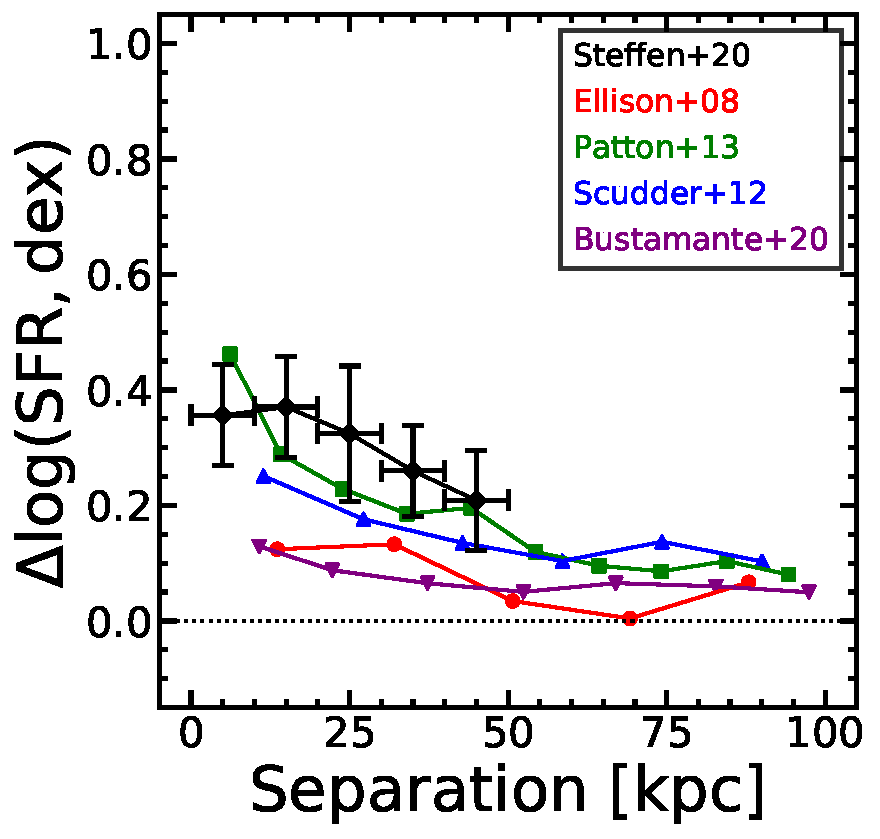
\includegraphics[width=3in]{fig/nuc_sep.pdf}
\caption[]{$\Delta$log(SFR) over projected separation for this sample (Black), \citet{Ellison:2008} (Red), \citet{Patton:2013} (Green), \citet{Scudder:2012} (Blue), and \citet{Bustamante:2020} (Purple). }
\label{fig:nuc_sep}
\end{figure}
%%%%%%%%%%%%%%%%%%%%%%%%%%%%%%%%%%%%%%%%%%%%%%

%%%%%%%%%%%%%%%%%%%%%%%%%%%%%%%%%%%%%%%%%%%%%%
\begin{figure}
\centering
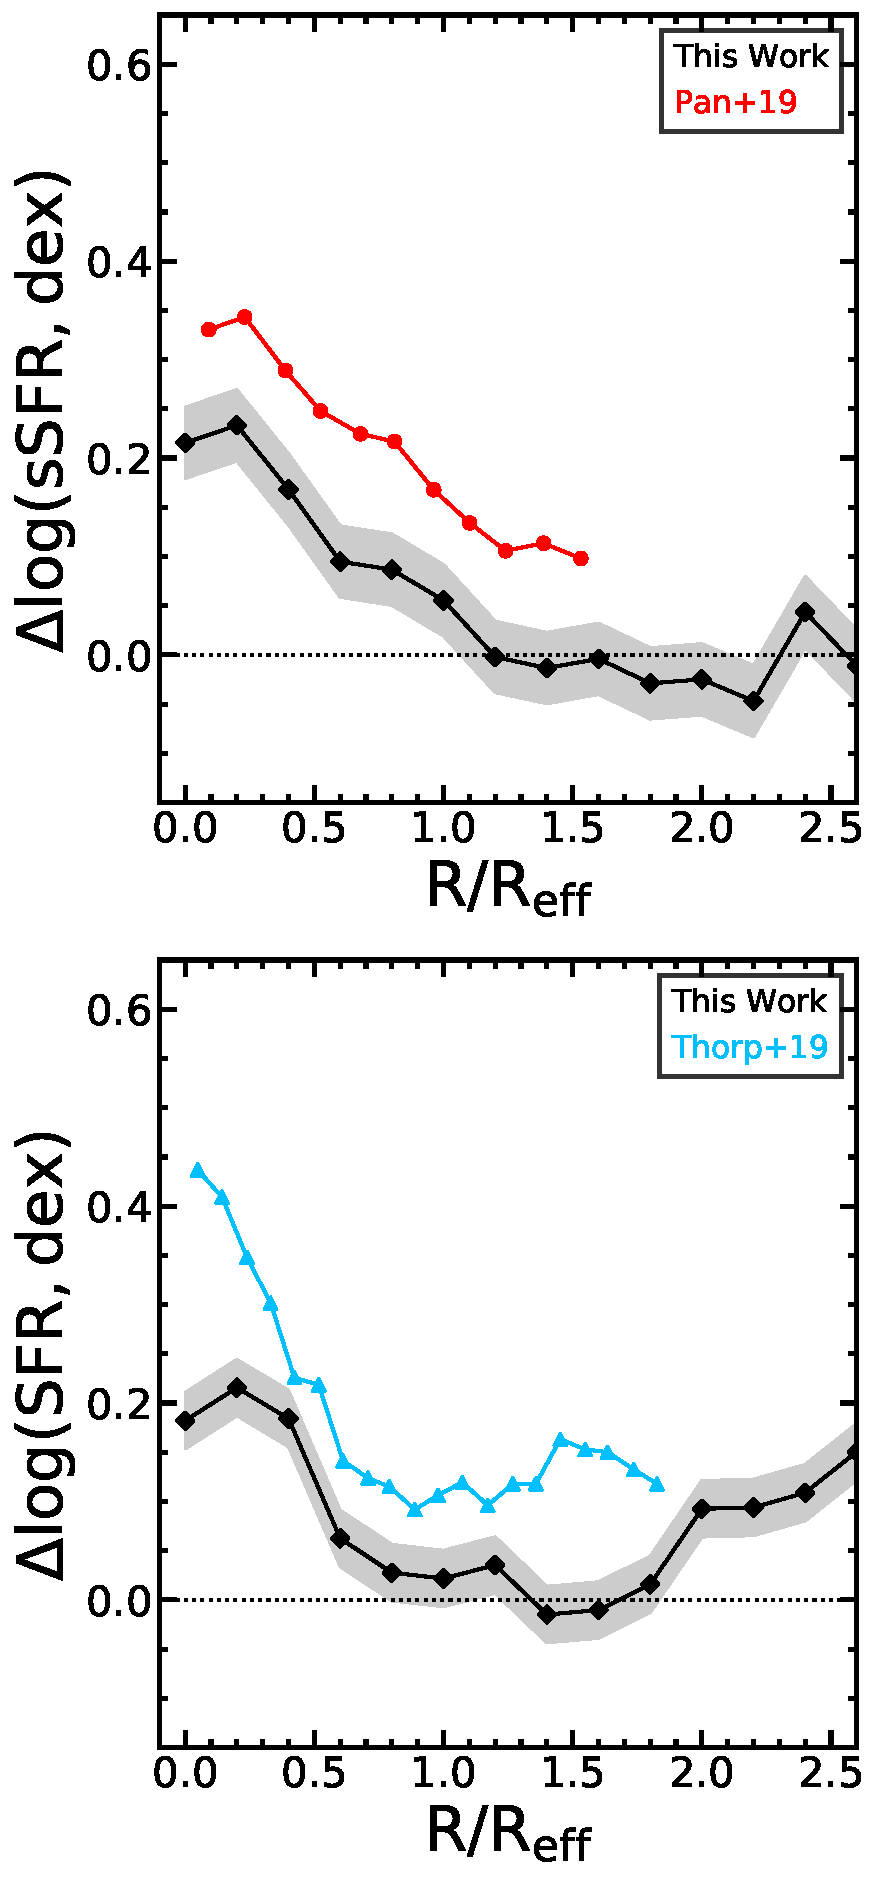
\includegraphics[width=3in]{fig/prof_comp.pdf}
\caption[]{The mean radial profile of $\Delta$log(sSFR) between pairs and controls of this work (red) compared against those of \citet{Pan:2019} (Blue) and \citet{Thorp:2019} (Green).}
\label{fig:prof_comp}
\end{figure}
%%%%%%%%%%%%%%%%%%%%%%%%%%%%%%%%%%%%%%%%%%%%%%

The $\Delta$log(SFR) as a function of projected separation has been studied before with the SDSS survey \citep{Ellison:2008, Patton:2013, Scudder:2012, Bustamante:2020}. We compare the mentioned surveys with our own work in Figure \ref{fig:nuc_sep}. We find that our pairs generally feature higher level of SFR enhancement in their centers, by $\sim$0.0$-$0.2 dex. Further, we probe galaxies with projected separations below 5 kpc, a projected separation range not covered in previous works. As mentioned in Section \ref{sec:sep}, we find a $\Delta$log(SFR) of zero implying that we are viewing galaxies that are about to or have just passed their first pericenter. 

Our sample only covers projected separations within 50 kpc, while previous surveys cover out to 100$-$200 kpc. While our sample covers a smaller separation range, the $\Delta$log(SFR) of our sample at 50 kpc is roughly the same level as \citet{Scudder:2012} and \citet{Patton:2013} at the same projected separation. This shows that the central SFR enhancement of our sample is consistent with with what has been found in previous works. 

In Figure \ref{fig:prof_comp} we look at the $\Delta$log(sSFR) profile as a function of galactocentric radius between our work and previous works. \citet{Pan:2019} examines a set of paired galaxies in the MaNGA survey while \citet{Thorp:2019} examines a set of post-merger galaxies in the MaNGA survey. The galaxy pairs in \citet{Pan:2019} have sSFR enhancements that are roughtly $\sim$0.05$-$0.2 dex higher than our sample. The $\Delta$log(sSFR) profile is closest to our work at the centers of the galaxy pairs but then begins to diverge further out into the galaxies' disks. Our paired galaxies show zero sSFR enhancement in their disks past 1.0 R/\reff\ while the galaxy pairs in \citet{Pan:2019} show an enhancement of $\sim$0.15 dex to the sSFR in their disks. 

The post-merger galaxies in \citet{Thorp:2019} have sSFR enhancements between $\sim$0.05$-$0.15 higher than our sample of paired galaxies. Their $\Delta$log(sSFR) profile follows our sample's profile closely between 0.25$-$1.0 R/\reff. The centers of the post-merger galaxies feature a greater level of sSFR enhancement in their centers compared to our galaxies pairs of $\Delta$log(sSFR) $=$ 0.5, roughly 0.25 dex higher than our paired galaxies. The post-merger galaxies also feature enhanced sSFR in their disk past 1.0 R/\reff\ of $\sim$0.1$-$0.15 dex. The heightened level of sSFR enhancement in the centers of post-merger galaxies in comparison to merging galaxies seems consistent with the idea that a second and greater burst of star formation occurs as the two merging galaxies coalesce into a single galaxy. 

\citet{Barrera-Ballesteros:2015} studied the sSFR in paired galaxies in the CALIFA IFS survey using the H$\alpha$ equivalent width (\ewha) as a proxy. They compared the sSFR in the centers of paired galaxies to their disks by varying the aperture diameters from which they extract the \ewha. They found that the sSFR is enhanced in the centers of the paired galaxies but suppressed in their disks. Between our work, \citet{Barrera-Ballesteros:2015}, and \citet{Pan:2019} there three is different scenarios; one where the disks of the paired galaxies see no change to the sSFR, one where the sSFR is suppressed, and one where the sSFR is enhanced. 

Looking at individual difference profiles in our work, we see that there is a large variance in the $\Delta$log(sSFR) where there are as many paired galaxies with sSFR enhancement in their disks as there are paired galaxies with suppression in there disks. The end result is that the average of the $\Delta$log(sSFR) is zero. The merger induced effects seen in the disks of the paired galaxies may be more complicated than what is seen in the centers of the galaxies. 


%%%%%%%%%%%%%%%%%%%%%%%%%%%%%%%%%%%%%%%%%%%%%%%%%%%%
\section{Summary and Conclusion}\label{sec:sum}

In this work, we studied a sample of paired, star forming galaxies using the MaNGA IFS survey. We have made a sample of 160 star forming galaxy pairs along with a set of 1891 star forming control galaxies. We compared the radial profiles of the paired galaxies with those of the controls galaxies and found the follwing;

\begin{enumerate}
\item The sSFR is centrally enhanced within the inner 1.0 R/\reff\ by 0.30 $\pm$ 0.1 dex. 
\item The disks of the paired galaxies, R/\reff\ $=$ 1.0$-$2.5, show no signs of either sSFR enhancement or sSFR suppression. 
\item The sSFR enhancement in paired galaxies is independent of the total stellar mass of the paired galaxies, Massive galaxies experience the same level of sSFR enhancement as low mass galaxies.
\item The sSFR enhancement in paired galaxies does depend on the ratio between the masses of the paired galaxies. Galaxies with small mass ratios, $|\Delta$log(M)$|$ $=$ 0.0$-$0.5, see an enhancement to sSFR of 0.4 $\pm$ 0.1 dex, which is 0.15 dex higher than the average paired galaxies in the survey. We have also showed that paired galaxies with large mass ratios, 1.0 $<$ $|\Delta$log(M)$|$ $<$ 2.0, still show substantial levels of enhancement to the sSFR, 0.1$-$0.2 dex. 
\item Further, in paired galaxies with large mass ratios, the less massive galaxies experience higher levels of sSFR enhancement than the more massive galaxy in the pair, $\sim$0.1 dex.
\item The sSFR enhancement increases with closer projected separations where galaxies within 5$-$15 kpc have their sSFR enhanced by 0.5$-$0.6 $\pm$ 0.1 dex. The galaxies within 5 kpc experience no central enhancement to their sSFR. We believe that these galaxies have just passed their first pericenter and the merger induced gas-inflow have yet to reach the centers of these galaxies.
\item The paired galaxies will experience a faster mass growth rate of secular evolution of 1.6$-$2.3$\times$. The growth rate is highest for massive galaxies; however, the the low mass galaxies will see a higher fractional mass increase in comparison to the preexisting stellar mass. 

\end{enumerate}

\acknowledgments

% funding
J.S. and H.F. acknowledge support from the National Science Foundation (NSF) grant AST-1614326 and University of Iowa funds. Funding for the Sloan Digital Sky Survey IV has been provided by the Alfred P. Sloan Foundation, the U.S. Department of Energy Office of Science, and the Participating Institutions. SDSS acknowledges support and resources from the Center for High-Performance Computing at the University of Utah. The SDSS web site is www.sdss.org.

SDSS is managed by the Astrophysical Research Consortium for the Participating Institutions of the SDSS Collaboration including the Brazilian Participation Group, the Carnegie Institution for Science, Carnegie Mellon University, the Chilean Participation Group, the French Participation Group, Harvard-Smithsonian Center for Astrophysics, Instituto de Astrofísica de Canarias, The Johns Hopkins University, Kavli Institute for the Physics and Mathematics of the Universe (IPMU) / University of Tokyo, the Korean Participation Group, Lawrence Berkeley National Laboratory, Leibniz Institut für Astrophysik Potsdam (AIP), Max-Planck-Institut für Astronomie (MPIA Heidelberg), Max-Planck-Institut für Astrophysik (MPA Garching), Max-Planck-Institut für Extraterrestrische Physik (MPE), National Astronomical Observatories of China, New Mexico State University, New York University, University of Notre Dame, Observatório Nacional / MCTI, The Ohio State University, Pennsylvania State University, Shanghai Astronomical Observatory, United Kingdom Participation Group, Universidad Nacional Autónoma de México, University of Arizona, University of Colorado Boulder, University of Oxford, University of Portsmouth, University of Utah, University of Virginia, University of Washington, University of Wisconsin, Vanderbilt University, and Yale University.

%%%%%%%%%%%%%%%%%%%% REFERENCES %%%%%%%%%%%%%%%%%%
\bibliographystyle{aasjournal}
\bibliography{mergerbib}

%%%%%%%%%%%%
% Appendix
%%%%%%%%%%%%

%\hbox{}\clearpage

%\appendix

%\section{Figures}

\end{document}